\documentclass[xcolor=table]{beamer}
\usepackage{graphicx}
\usepackage[spanish]{babel} % para escribir en espanol
\usepackage[utf8]{inputenc}
\usepackage{wrapfig}
\usepackage{listings}

\graphicspath{ {imagenes/} }

\usetheme{Madrid}

\lstset{language=R,
           basicstyle=\ttfamily,
           keywordstyle=\color{blue}\ttfamily,
           stringstyle=\color{red}\ttfamily,
           commentstyle=\color{green}\ttfamily,
           breaklines=true
          }

\title{Aplicaciones del análisis multivariante con R}
\subtitle{Estadística Multivariante - Universidad de Granada}

\author{Laura Gómez Garrido\\ Miguel Lentisco Ballesteros \\ Antonio Martín Ruiz \\ Daniel Pozo Escalona \\Francisco Javier Sáez Maldonado}

\AtBeginSection[]
{
  \begin{frame}<beamer>{}
    \tableofcontents[currentsection,currentsubsection]
  \end{frame}
}

\begin{document}
\begin{frame}
\titlepage
\end{frame}
\begin{frame}{Contenido}
  \tableofcontents
  % You might wish to add the option [pausesections]
\end{frame}
\section{Introducción: R}

\begin{frame}{¿Qué es R?}
\begin{wrapfigure}{r}{0.4\textwidth}
\centering

\includegraphics[width=0.4\textwidth]{r.png}
\end{wrapfigure}{
R es un entorno y lenguaje de programación enfocados a la computación
estadística y de gráficos. Surge como una reimplementación libre del lenguaje y
entorno S. Proporciona una amplia variedad de funcionalidades estadísticas y
gráficas y es altamente extensible.}

\end{frame}

\begin{frame}
  
R está disponible como software libre bajo los términos de la GNU General Public
License de la Free Software Foundation en forma de código fuente. Puede ser
compilado y ejecutado en una gran cantidad de plataformas UNIX, Windows y MacOs.

\end{frame}

\begin{frame}{Librerías y paquetes}
R forma parte de un proyecto colaborativo y abierto donde sus propios usuarios pueden publicar paquetes.
\newline
\newline
\begin{wrapfigure}{r}{0.4\textwidth}
\centering

\includegraphics[width=0.4\textwidth]{r-forge.png}
\end{wrapfigure}
{Utiliza la forja de desarrollo R-Forge.}
\newline
\newline
{En Diciembre de 2019, el repositorio oficial tenía disponibles 15.315 paquetes organizados en vistas o temas. }
\end{frame}

\begin{frame}[fragile]{Cómo instalar dependencias}
R incluye un gestor de paquetes integrado en el lenguaje, que permite instalar dependencias con la orden \texttt{install.packages()}.
  
\begin{lstlisting}[language=R, basicstyle=\ttfamily]
install.packages("MVA")
install.packages("HSAUR2")
install.packages("car")
install.packages("MASS")
\end{lstlisting}

\end{frame}

\begin{frame}[fragile]{Cómo instalar dependencias}
Para importar los paquetes para usarlos en un programa:  
\begin{lstlisting}[language=R, basicstyle=\ttfamily]
library("MVA")
library("HSAUR2")
library("car")
library("MASS")
\end{lstlisting}

\end{frame}

\begin{frame}{Algunas vistas}

\begin{itemize}
\begin{minipage}{0.45\textwidth}
\item Bayesian
\item ChemPhys
\item ClinicalTrials
\item Cluster
\item Databases
\item DiferrentialEquations
\item Distribution
\item Genetics
\item MachineLearning
\item Multivariate
\end{minipage}
\begin{minipage}{0.45\textwidth}
\begin{minipage}{\textwidth}

\includegraphics[width=0.65\textwidth]{aefi.png}
\vspace{1cm}
\end{minipage}
\begin{minipage}{\textwidth}
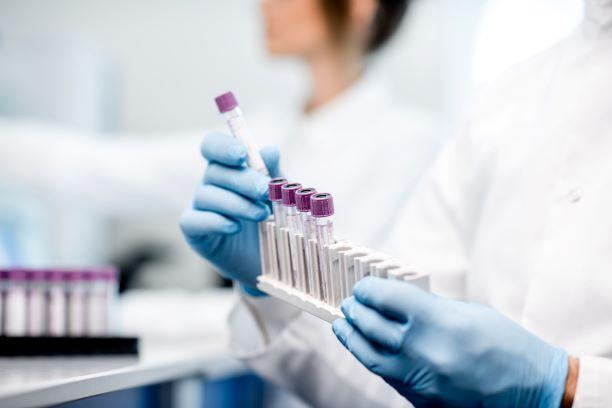
\includegraphics[width=0.65\textwidth]{ensayo.jpg}
\vspace{1cm}
\end{minipage}
\begin{minipage}{\textwidth}

\includegraphics[width=0.65\textwidth]{genetica.jpg}
\end{minipage}
\end{minipage}
\end{itemize}
\end{frame}

\section{R en el análisis multivariante}
\begin{frame}{Nuestro dataset}

\begin{table}[]
\resizebox{10cm}{!}{
\begin{tabular}{|
>{\columncolor[HTML]{979CD8}}l |l|
>{\columncolor[HTML]{979CD8}}l |l|}
\hline
\textbf{Característica del data set}      & Multivariante   & \textbf{Nº de Instancias} & 178        \\ \hline
\textbf{Características de los atributos} & Enteros, Reales & \textbf{Nº de Atributos}  & 13         \\ \hline
\textbf{Área}                             & Física          & \textbf{Donado}           & 01/07/1991 \\ \hline
\end{tabular}
}
\end{table}
\begin{wrapfigure}{r}{0.25\textwidth}
\centering
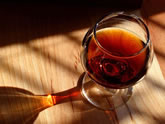
\includegraphics[width=0.2\textwidth]{vino.jpg}
\end{wrapfigure}
{Fuente: Machine Learning Repository\\
Propietarios Originales: }\begin{quote}\scriptsize Forina, M. et al, PARVUS -\\
An Extendible Package for Data Exploration, Classification \\and Correlation.\\
Institute of Pharmaceutical and Food Analysis and Technologies, \\Via Brigata Salerno,
16147 Genoa, Italy.\end{quote}
\end{frame}


\subsection{Distribución Normal Multivariante. Ejemplos}

\begin{frame}[fragile]{Lectura}



\begin{lstlisting}[language=R, basicstyle=\ttfamily]
wine <- read.table("http://archive.ics.uci.edu/ml/machine-learning-databases/wine/wine.data",sep=",")
\end{lstlisting}
\centering
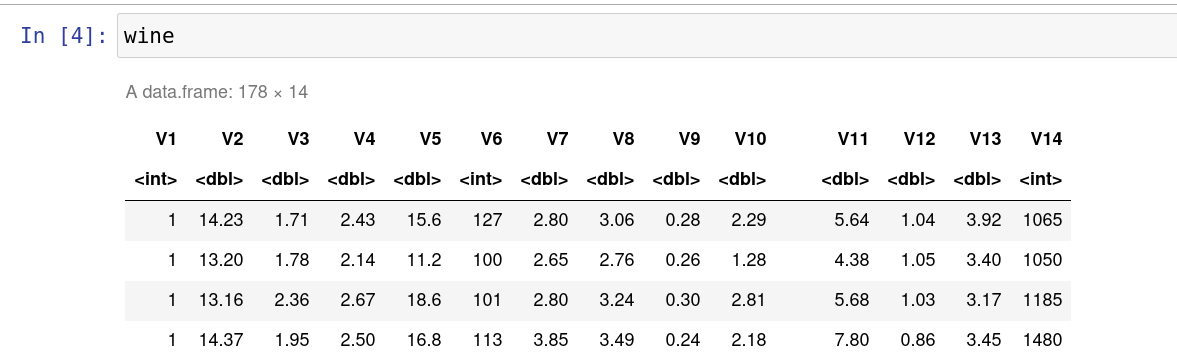
\includegraphics[width=0.8\textwidth]{dataframe_wine.png}

\begin{itemize}
\item $read.csv$ o $read.csv2$
\item $read.delim$
\end{itemize}
\end{frame}



\begin{frame}[fragile]{Media y desviación típica. Normalización.}
    \begin{columns}[c] % the "c" option specifies center vertical alignment
    \column{.5\textwidth} % column designated by a command
     \begin{lstlisting}[language=R, basicstyle=\ttfamily]
sapply(wine[2:14],mean)
V2 13.0006179775281
V3 2.33634831460674
...
V13 2.61168539325843
V14 746.893258426966 
\end{lstlisting}
    \column{.5\textwidth}
     \begin{lstlisting}[language=R, basicstyle=\ttfamily]
sapply(wine[2:14],sd)
V2 0.811826538005857
V3 1.11714609761446
...
V13 0.70999042876505
V14 314.907474276849
\end{lstlisting}



    \end{columns}
    \begin{lstlisting}[language=R, basicstyle=\ttfamily]
    standardised_wine <- as.data.frame(scale(wine[2:14]))
\end{lstlisting}
\end{frame}


\begin{frame}[fragile]{Ejemplo de selección de datos}
\begin{lstlisting}
selection1 <- wine[wine$V1 == "1",]
selection3 <- wine[wine$V1 == "3",]
mean1 <- sapply(selection1[2:14],mean)
mean2 <- sapply(selection3[2:14],mean)
chemical <- c(2,3,4,5,6,7,8,9,10,11,12,13,14)
plot(chemical,mean1,col = "red")
points(chemical, mean2, col="blue", pch="*")
legend(2,1000,legend=c("Medias en Fabrica 1","Medias en Fabrica 2"), col=c("red","blue"),
                                   pch=c("o","*"))
\end{lstlisting}

\begin{wrapfigure}{r}{0.25\textwidth}
\centering
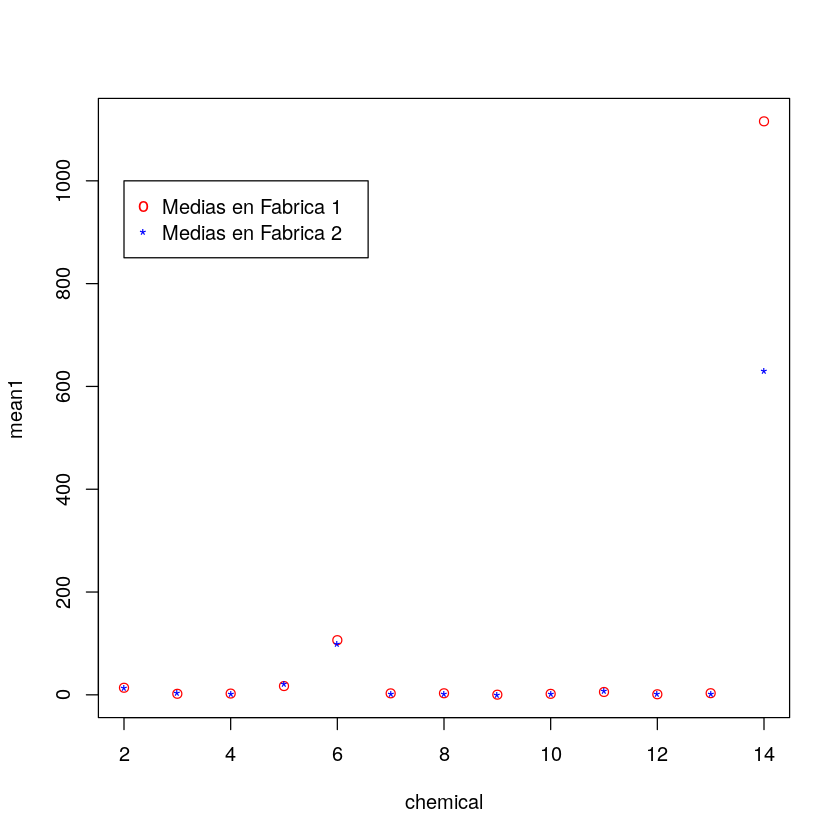
\includegraphics[width=0.8\textwidth]{means.png}
\end{wrapfigure}
\end{frame}
\subsection{Scatterplots}
\begin{frame}[fragile]{Scatterplots}

Podemos realizar scatterplots de la siguiente manera



\begin{lstlisting}
plot(popul ~ manu, data = USairpollution)
\end{lstlisting}
\centering
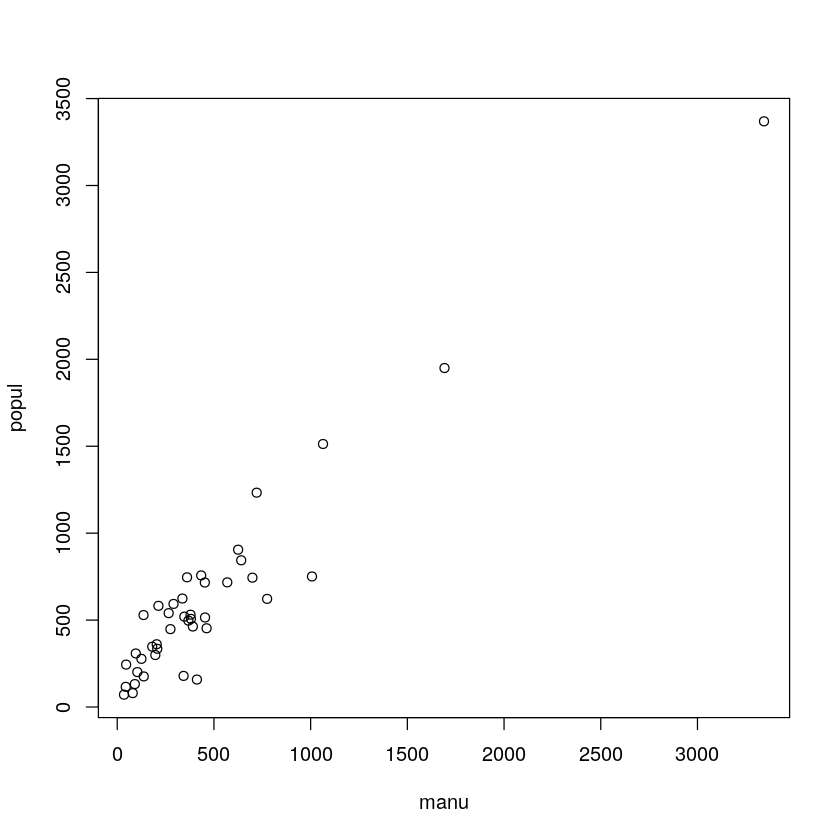
\includegraphics[width=0.4\textwidth]{scatter.png}



\end{frame}
\begin{frame}[fragile]
O, dibujar todas las parejas posibles a la vez, y añadir las rectas de regresión

\begin{lstlisting}
pairs(USairpollution,
     panel = function(x, y, ...) {
         points(x, y, ...)
         abline(lm(y ~ x), col = "grey")
     }, pch = ".", cex = 1.5)
\end{lstlisting}
\end{frame}
\begin{frame}
\centering
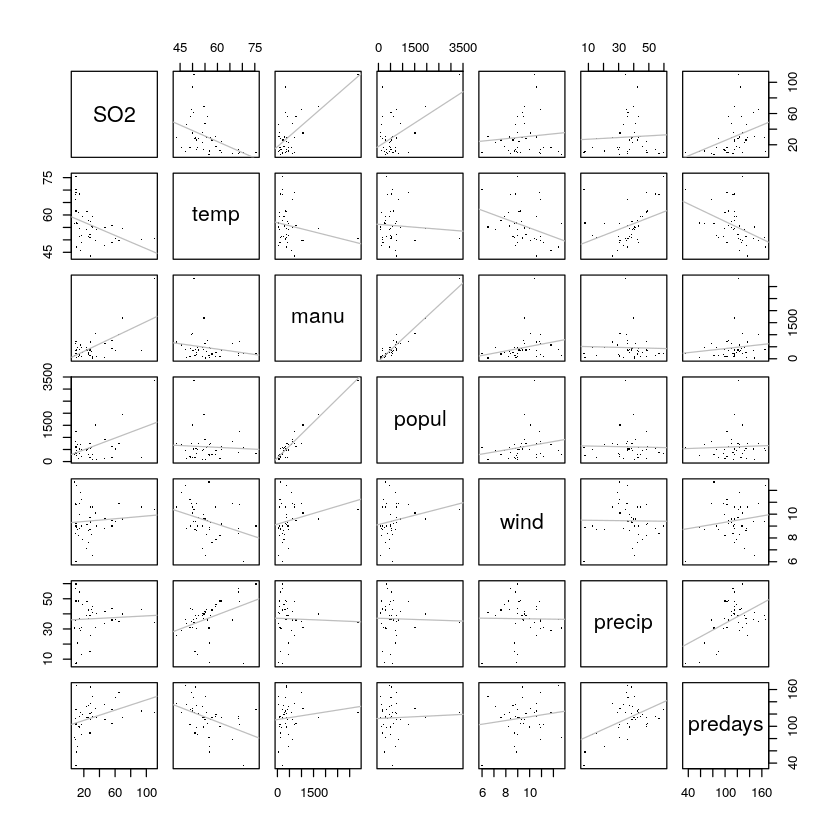
\includegraphics[width=0.7\textwidth]{reg.png}
\end{frame}


\begin{frame}[fragile]{Implementación Teórica de una DNM}

\begin{lstlisting}
DNM <- setRefClass("DNM", 
                   fields = list(p = "numeric", 
                                 media = "matrix", 
                                 cov = "matrix"))
\end{lstlisting}
\end{frame}

\begin{frame}[fragile]{Ejemplo de creación de una DNM}
$\pmb{X} = (X_1, X_2, X_3)^T \sim N_3 \begin{pmatrix} \begin{pmatrix} 2 \\ 3 \\ -1 \end{pmatrix}, && \begin{pmatrix} 1 & 0 & 1 \\ 0 & 5 & -2 \\ 1 & -2 & 2 \end{pmatrix} \end{pmatrix} $

\begin{lstlisting}

means <- matrix(c(2,3,-1), nrow = 3, ncol = 1)

cov <- matrix(c(1, 0, 1, 0, 5, -2, 1, -2, 2), nrow = 3, ncol = 3)

X <- DNM$new(p = 3, media = means, cov = cov); X

t(chol(X$cov)) \%*\% (chol(X$cov))

\end{lstlisting}
\end{frame}

\begin{frame}[fragile]{Función de densidad}
  \begin{lstlisting}
    # Pre: X es DNM, x matriz
funcion_densidad <- function(X, x) {
    if (dim(x)[1] != X$p)
        stop("Filas de x no coinciden con dimension de X")
    if (dim(x)[2] != 1)
        stop("x no es vector columna")
    if (det(X$cov) <= 0)
        stop("Matriz de covarianzas no es definida positiva")
    # f_X(x)
    exp(-0.5 * as.numeric(t(x - X$media) %*% solve(X$cov) %*% (x - X$media))) / ((2 * pi)^(X$p / 2) * sqrt(det(X$cov)))
}
  \end{lstlisting}
\end{frame}

\begin{frame}[fragile]{Función característica}
  \begin{lstlisting}
# Pre: X es DNM, t es matriz
funcion_caracteristica <- function(X, t) {
    # Comprobacion de rango
    if (dim(t)[1] != X$p)
        stop("Filas de t no coinciden con dimension de X")
    if (dim(t)[2] != 1)
        stop("t no es vector columna")
    # psi_X(t)
    exp(as.complex(1i * t(t) %*% X$media - 0.5 * t(t) %*% X$cov %*% t))
}
  \end{lstlisting}
\end{frame}

\begin{frame}[fragile]{Teorema de la transformación lineal}
Necesita como argumentos una DNM $\pmb{X} \sim N_p(\pmb{\mu}, \Sigma)$, una matriz $B \in \mathcal{M}_{qxp}$ ($q \leq p$) y un vector $\pmb{b} \in \mathbb{R}^q$. Entonces devuelve la DNM definida como $\pmb{Y} = B \pmb{X} + \pmb{b}$, entonces $\pmb{Y} \sim N_q(B \pmb{\mu} + \pmb{b}, B \Sigma B^T)$, con $B\Sigma B^T > 0$.

\begin{lstlisting}
transformacion_lineal <- function(X, B, b) {
    # Comprobaciones de rango
    if (dim(B)[1] > dim(B)[2])
        stop("Dimension de B incorrecta (q > p)")
    if (dim(B)[2] != X$p)
        stop("Columnas de B no coinciden con dimension de X")
    if (dim(b)[1] != dim(B)[1])
        stop("Filas de B no coinciden con dimension de b")
    if (dim(b)[2] != 1)
        stop("b no es un vector columna")
    # Nueva DNM
    media_y = matrix(B \%*\% X$media + b, ncol = 1)
    cov_y = matrix(B \%*\% X$cov \%*\% t(B), nrow = dim(B)[1])
    DNM\$new(p = dim(B)[1], media = media_y, cov = cov_y)
}
\end{lstlisting}
\end{frame}

\section{Para ampliar}
\begin{frame}{Para ampliar}
\textit{Computing Machinery and Intelligence} Alan Turing (1950)
\newline
\newline
\textit{Artifficial Intelligence: A Modern Aproach} Stuart J. Russell y Peter Norvig
\newline
\newline
\textit{Concrete Problems in AI Safety} Dario Amodei, Crhis Olah, Jacob Steinahrdt, Paul Christiano, John Schulman, Dan Mané
\newline
\newline
\textit{The Malicious Use of Artificial Intelligence: Forecasting, Prevention, and Mitigation} Miles Brundage, Shahar Avin et al.
\end{frame}
\end{document}
